As described in the problem statement, the primary objective of the Google Books
project is to create a digital library with global accessibility.~Through
collaborations with libraries and publishers worldwide, the project has amassed
a collection of over 40 million books in more than 400 languages. The process of
adding a book to the digital library involves several key steps, such as library
registration, on-site visits by logistics experts, and shipping the books for
scanning. Therefore, the development of an efficient scanning process requires
careful planning for optimal efficiency.~Motivated by these real-world
challenges, this problem presents a scenario that resembles the real-world
challenges face by the Google Books team.

In the context of this problem, we are presented with a global library system
housing a diverse collection of books, with each library having at most one copy
of these books.~Libraries are characterized by three key factors: the books they
hold, sign-up time, and shipping rate. The sign-up time represents the duration
(measured in days) required for a library to complete the sign-up process before
it can commence sending books for scanning. The shipping rate indicates how many
books a library can send for scanning daily once the sign-up process concludes.
Henceforth, given a number of libraries denoted as~$\mathcal{L}$, we shall
use the notation~$t_{\ell}$ and~$r_{\ell}$ to refer to the sign-up time of a
library,~$\ell = 1, \ldots, \mathcal{L}$, respectively.

There are specific constraints associated with tThe book scanning process, as
described, is nevertheless limited by time as there is a fixed global
deadline,$\mathcal{D}$. Consequently, it is likely that only a portion of all
available libraries will undergo the sign-up process.  Moreover, for the
libraries that are already signed up, this deadline restricts the number of days
during which they are allowed to ship books for scanning.~Firstly,
only one library can be signed-up at any given time, irrespective of any
predefined order. Moreover, once the sign-up process commences for a particular
library, it cannot be halted, and as soon as it concludes, that library becomes
immediately available for sending books for scanning. Notably, each book scanned
contributes a designated score; however, this score is counted only once,
regardless of how many times the book is scanned. Given a number of
books,~$\mathcal{B}$, the notation $s_{b}$ will be used to denote the score of
book~$b = 1, \ldots, \mathcal{B}$.

The book scanning process, as described, is nevertheless limited by time as
there is a fixed global deadline,~$\mathcal{D}$.~Consequently, it is likely that
only a portion of all available libraries will undergo the sign-up process.
Moreover, for the libraries that are already signed up, this deadline restricts
the number of days during which they are allowed to ship books for scanning.

As an illustrative example, refer to~\Cref{fig:bs-example}, which depicts a
possible book scanning process.~The characteristics of the libraries in the
example are detailed in~\Cref{tab:bs-library-properties}. It is important to
note that, in this specific example, the global deadline has been set at 7 days
(inclusive).

\begin{figure}[h]
  \centering
  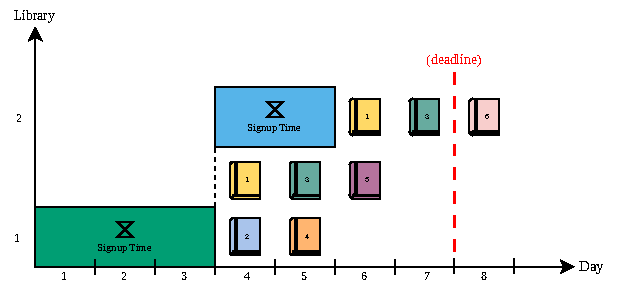
\includegraphics[width=\textwidth,keepaspectratio]{../assets/bs/bs-example.pdf}
  \caption{Book Scanning Process Example}
  \label{fig:bs-example}
\end{figure}

\begin{table}[ht]
  \centering
  \begin{tabular}{cccc}
  \toprule
  Library & Sign-up Time & Rate & Books         \\
  \midrule
  1       & 3            & 2    & 1, 2, 3, 4, 5 \\
  2       & 2            & 1    & 1, 3, 6       \\
  \bottomrule
\end{tabular}
  \caption{Library Properties}
  \label{tab:bs-library-properties}
\end{table}

In this specific example, two libraries have signed up in a non-decreasing order
based on their labels, resulting in a combined sign-up time of 5 days.
Additionally, the scanning rates for these libraries are 2 and 1 for library 1
and 2, respectively. This implies that with this library order, library 1 can
ship a maximum of 8 books, while library 2 can ship 2 books at
most.~Consequently, the latter ends up not contributing one of its books to the
scanning process.~Importantly, this example also highlights a scenario where
both libraries possess duplicate copies of the same books (books 1 and 3).~As
mentioned earlier, these duplicate copies will only be scanned once, regardless
of the number of duplicates, ensuring that they are counted for scoring only
once.

In essence, the objective of this problem is to determine the optimal order for
library sign-ups and book selections for scanning, aiming to maximize the sum of
the scores of the unique books sent for scanning before the deadline.
Mathematically, this can be expressed as shown in~\Cref{eq:bs-objective}, where,
$\mathcal{I}$ the number of libraries signed-up, $\phi^\mathcal{I}$ denotes the
order for the signed-up libraries $i = 1, \ldots, \mathcal{I}$, and $x_{b,l}$ is
a binary variable indicating whether a particular book, $b$, was shipped by
library $\ell$ for scanning (1) or not (0).

\begin{equation}
  \label{eq:bs-objective}
  \begin{aligned}
    \max{f(x)} =\  & \sum_{b = 1}^{\mathcal{B}}{s_{b} \cdot \min\left(\sum_{i = 1}^{\mathcal{I}}{x_{b, \phi_{i}^\mathcal{I}}} , 1\right)}                                                                     \\
    \text{s.t }    & \sum_{b = 1}^{\mathcal{B}}{x_{b, \phi_{i}^\mathcal{I}}} \leq r_{i} \cdot \left(\mathcal{D} - \sum_{k = 1}^{i}{t_{\phi_{k}^\mathcal{I}}} \right) \quad \forall i = 1, \ldots, \mathcal{I} \\
                   & \sum_{i = 1}^{\mathcal{I}}{t_{\phi_{i}^\mathcal{I}}} \leq \mathcal{D}                                                                                                                    \\
  \end{aligned}
\end{equation}

Note that in the objective function given by~\Cref{eq:bs-objective}, the
constraints represent the maximum number of books that a library can ship for
scanning between its sign-up date and the deadline, as well as the maximum
number of libraries that can undergo the sign-up process before the deadline.

For clarification of all the above concepts, consider the books scores presented
in~\Cref{tab:bs-example}.

\begin{table}[ht]
  \centering
  \begin{tabular}{ccccccc}
  \toprule
  \textbf{Book}  & 1 & 2 & 3 & 4 & 5 & 6 \\ \midrule
  \textbf{Score} & 3 & 1 & 5 & 4 & 7 & 1 \\
  \bottomrule
\end{tabular}
  \caption{Example Book Scores}
  \label{tab:bs-example}
\end{table}

Given the order for the libraries shown in~\Cref{fig:bs-example} and the
properties exposed in~\Cref{tab:bs-library-properties} the resulting objective
value for this scheduling is~$3 + 1 + 5 + 4 + 7 = 20$.

Lastly, several instance-specific constraints are applied to various parameters
that define the data center design within the context of this problem. These
constraints are as follows:

\begin{description}
  \item[\textbf{$\mathcal{L}$.}] The number of libraries~($ 1 \leq \mathcal{L} \leq 10^5$).
  \item[\textbf{$\mathcal{T}$.}] The number of days required to finish a library sign-up~($ 1 \leq \mathcal{T} \leq 10^5$).
  \item[\textbf{$\mathcal{B}$.}] The number of unique books~($ 1 \leq \mathcal{B} \leq 10^5$).
  \item[\textbf{$\mathcal{N}$.}] The number of books per library~($ 1 \leq \mathcal{N} \leq 10^5$).
  \item[\textbf{$\mathcal{D}$.}] The deadline~($ 0 \leq \mathcal{D} \leq 10^5$).
\end{description}